% !TeX root = ../tese_modelo.tex
\chapter{[Título do Capítulo]}
\label{ch:modelo}

[Parágrafo de apresentação do capítulo: o que será tratado, por que importa para o trabalho e como o capítulo se organiza.] \cite{chave2024exemplo}.

\section{[Título da Seção]}
\label{sec:modelo_secao}

Texto corrido com valor numérico e unidade, como $1{,}5$~m de comprimento e $20$~kg de massa. Citação com autor na frase: conforme \citeonline{chave2024exemplo}. Referências cruzadas: \autoref{tab:modelo}, \autoref{fig:modelo}, \autoref{eq:modelo} e \aref{ap:modelo}.

\begin{equation}
	y = a\,x + b,
	\label{eq:modelo}
\end{equation}
onde $y$ é a variável dependente, $x$ a variável independente, $a$ o coeficiente angular e $b$ o coeficiente linear.

\begin{table}[h!]\centering
	\setlength{\tabcolsep}{8pt}
	\renewcommand{\arraystretch}{1.2}
	\caption[Título curto da tabela]{Legenda completa da tabela. Elaborado pelo autor.}\label{tab:modelo}
	\small
	\begin{tabular}{M{2,4cm}M{4,2cm}M{2,4cm}}\toprule
		\textbf{Coluna A} & \textbf{Coluna B} & \textbf{Coluna C} \\
		\midrule
		$1{,}0$ & texto & $2{,}5$~kg \\
		\bottomrule
	\end{tabular}
\end{table}

\begin{figure}[h!]
	\centering
	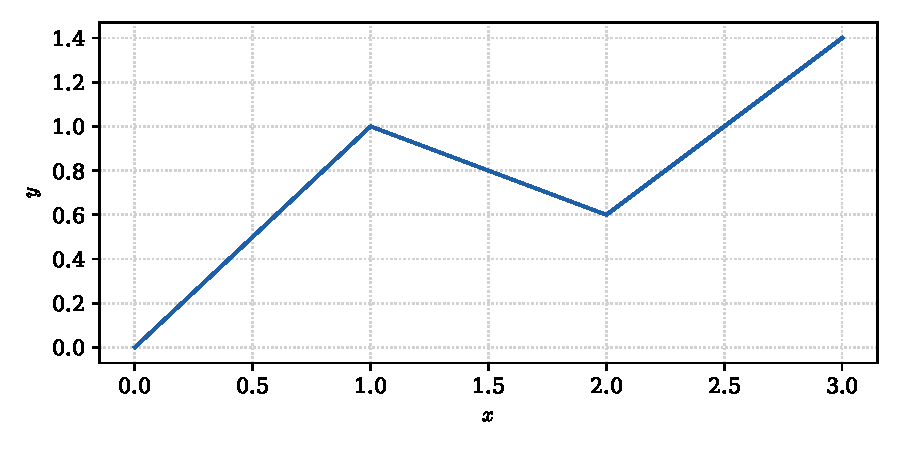
\includegraphics[width=0.95\linewidth]{figuras/exemplo.pdf}
	\caption[Título curto da figura]{Legenda completa da figura. Elaborado pelo autor.}
	\label{fig:modelo}
\end{figure}

\begin{figure}[h!]
	\centering
	\begin{subfigure}[b]{0.49\linewidth}\centering
		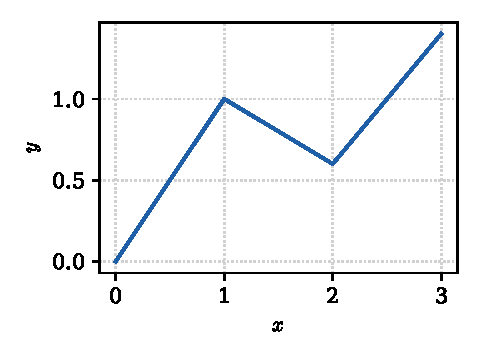
\includegraphics[width=\linewidth]{figuras/exemplo_a.pdf}
		\caption{Painel A}\end{subfigure}\hfill
	\begin{subfigure}[b]{0.49\linewidth}\centering
		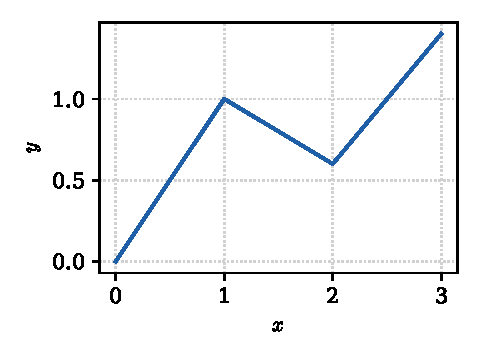
\includegraphics[width=\linewidth]{figuras/exemplo_b.pdf}
		\caption{Painel B}\end{subfigure}
	\caption[Título curto das subfiguras]{Legenda geral das subfiguras. Elaborado pelo autor.}
	\label{fig:modelo_sub}
\end{figure}

\section{\novo{[Seção com Texto Novo]}}
\label{sec:modelo_novo}

\novo{Texto recém-inserido, em vermelho até a aprovação.} \preencher{informação pendente}
